\documentclass{ieeeaccess}
\usepackage{cite}
\usepackage{amsmath,amssymb,amsfonts}
\usepackage{graphicx,textcomp,bm}
\usepackage{booktabs,tabularx,array,multirow}
\usepackage{seqsplit}
\newcolumntype{Y}{>{\centering\arraybackslash}X}
\begin{document}
\vol{14}
\year{2026}
\history{Supplementary material revised September 7, 2026.}
\doi{10.1109/ACCESS.2026.0000000}
\title{Supplementary Material for ``DiSwitch''}
\author{\uppercase{Kyung Eun Kim}\authorrefmark{1} and \uppercase{Howon Lee}\authorrefmark{1}}
\address[1]{Department of Military Digital Convergence, Ajou University, Suwon 16499, Republic of Korea}
\markboth{K. E. Kim and H. Lee: Supplementary Material for DiSwitch}{K. E. Kim and H. Lee: Supplementary Material for DiSwitch}
\corresp{Corresponding author: Howon Lee.}
\begin{abstract}
This supplementary document records experimental provenance, metric semantics, statistical units, reliability acceptance gates, negative results, and the complete 20-figure latency and reliability portfolio supporting the DiSwitch article. It also provides the DiSwitch-versus-Fast-DiSwitch gate table, operator-profile interpretation, and a reproduction and submission checklist.
\end{abstract}
\begin{keywords}
FANET, inference latency, reproducibility, supplementary material, UAV routing.
\end{keywords}
\titlepgskip=-21pt
\maketitle

\section{Artifact and Provenance Inventory}

Table~\ref{tab:inventory} maps each claim family to its authoritative local artifact. Paths are relative to the project root. This IEEE Access package copies publication-facing tables and figure sources into \texttt{\seqsplit{paper/diswitch\_ieee\_access}}; the immutable experiment folders remain the source of record.

\begin{table*}[t]
\caption{Evidence inventory.}\label{tab:inventory}\small
\begin{tabularx}{\textwidth}{p{0.19\textwidth}p{0.43\textwidth}X}
\toprule
Claim family & Authoritative artifact & Scope and caveat \\
\midrule
Eight-method routing comparison & R1 & 112,000 episode rows; five seeds; 14 scenarios; scenario-macro statistics \\
DiSwitch--Fast-DiSwitch reliability & R2 & Paired seed differences; predeclared 0.5 percentage-point non-inferiority floor \\
A100 latency & R3 & Same A100 session; batch 1; warm-up 50; 2,000 repeats; five checkpoints \\
Operator attribution & R4 & Seed 42; held-out medium; 30 profiled calls; not the primary latency sample \\
Early-exit behavior & R5 & 43,467 decisions; 14,000 paired episodes; empirical, not formal, equivalence \\
Method implementation & R6 & Canonical alias SwitchGlobePolicy; unified decide() path \\
Literature corpus & R7 & 45 accessible Notion database records; metadata audit, not meta-analysis \\
\bottomrule
\end{tabularx}
\end{table*}

\noindent\textbf{Artifact keys.} R1: \seqsplit{artifacts/final\_paper\_simulation/synthesis/combined\_comparison/}; R2: \seqsplit{artifacts/final\_paper\_simulation/full/ablation/validation/fast\_vs\_exact\_overall.csv}; R3: \seqsplit{artifacts/switchglobe\_latency\_optimization/globev2\_colab\_cli\_20260905/results/}; R4: the sibling \seqsplit{profile/results/} directory; R5: \seqsplit{docs/latency\_optimization/final\_report.md}; R6: \seqsplit{implementations/lite\_globe/models/student\_policy.py}; R7: \seqsplit{paper/diswitch\_ieee\_access/literature\_comparison.csv}.

The combined manifest reports completion, 112,000 episode rows, 560 seed summaries, and exact cross-experiment row matching. It also records that the source worktree contained dirty files when the archive was synthesized. That disclosure is retained as a limitation. Before public release, the authors should rebuild the final archive from a clean tag and publish the commit, environment lock, and hashes together.

\section{Metric Definitions and Statistical Unit}

The primary reliability metric is connected-pair packet delivery ratio (PDR), which conditions on source--destination pairs that were initially connected. Overall PDR retains all episodes and therefore mixes routing failure with initial disconnection. Deadline delivery counts packets delivered within the simulator deadline. Successful-delay metrics condition on delivery; cells with no delivered packets are undefined and must be displayed as N/A rather than zero.

The simulator energy quantity is a proxy, not joules. The scenario-macro synthesis includes its documented failure treatment, whereas another pooled analysis uses a different weighting. Results in the manuscript and this supplement consistently follow the synthesis files. Policy-input bytes measure input tensor memory, not HELLO messages, route requests, eBPF update bytes, or total radio overhead.

The seed is the inferential unit. Individual episodes and individual timing repetitions reveal distributions but do not replace independent training seeds. With five seed pairs, a two-sided exact sign-flip test has minimum attainable $p=0.0625$; effect size and confidence interval are therefore reported alongside the exact test.

\section{Complete Figure Portfolio}

Each figure below has a publication PNG and vector SVG in the supplementary-figure directory. Its plotted values are stored in a correspondingly numbered CSV in \texttt{figure\_data}. Captions distinguish local CPU, current A100, older A100 evidence, full reliability, and diagnostic-only episode timing.

\begin{figure*}[t]\centering

\includegraphics[width=0.92\textwidth]{supplementary_figures/01_baseline_component_latency.png}
\caption{Independent component timers for the local batch-one policy path over five seeds. Components are measured separately for bottleneck diagnosis and must not be summed to recreate the end-to-end timer.}
\label{fig:s01}\end{figure*}

\begin{figure*}[t]\centering

\includegraphics[width=0.92\textwidth]{supplementary_figures/02_latency_summary.png}
\caption{Mean, median, p95, and p99 latency summaries for DiSwitch and candidate variants. Fast-DiSwitch variants are approximate policies and require a separate reliability judgment.}
\label{fig:s02}\end{figure*}

\begin{figure*}[t]\centering

\includegraphics[width=0.90\textwidth]{supplementary_figures/03_latency_ecdf.png}
\caption{Empirical distribution of five seed-specific p95 values. It avoids presenting thousands of correlated routing decisions as independent experimental replications.}
\label{fig:s03}\end{figure*}

\begin{figure*}[t]\centering

\includegraphics[width=0.90\textwidth]{supplementary_figures/04_latency_forest.png}
\caption{Paired p95 speed effects. Positive is faster than DiSwitch. Confidence intervals are computed across matched checkpoints.}
\label{fig:s04}\end{figure*}

\begin{figure*}[t]\centering

\includegraphics[width=0.90\textwidth]{supplementary_figures/05_pareto_connected_pair_pdr.png}
\caption{Connected-pair PDR versus A100 decision latency. Reliability and latency originate from separate, explicitly scoped experiments: the full routing evaluation and the same-session microbenchmark.}
\label{fig:s05}\end{figure*}

\begin{figure*}[t]\centering

\includegraphics[width=0.90\textwidth]{supplementary_figures/06_pareto_deadline_delivery_ratio.png}
\caption{Deadline-delivery ratio versus A100 p95 decision latency. DiSwitch occupies the reliability-oriented point; Fast-DiSwitch occupies a lower-latency but lower-reliability point.}
\label{fig:s06}\end{figure*}

\begin{figure*}[t]\centering

\includegraphics[width=\textwidth]{supplementary_figures/07_reliability_heatmap.png}
\caption{Scenario-level reliability heatmap. It reveals that Fast-DiSwitch degradation is concentrated in specific OOD node-density and predictive-break conditions rather than uniform across the benchmark.}
\label{fig:s07}\end{figure*}

\begin{figure*}[t]\centering

\includegraphics[width=\textwidth]{supplementary_figures/08_latency_heatmap.png}
\caption{Diagnostic latency collected during the full 14,000-episode routing execution. It is useful for scenario localization but is not a same-session randomized microbenchmark and is not used as the primary A100 estimate.}
\label{fig:s08}\end{figure*}

\begin{figure*}[t]\centering

\includegraphics[width=\textwidth]{supplementary_figures/09_seed_variability.png}
\caption{Seed-level variability for all optimized candidates. Matching seeds across variants enables paired rather than unpaired effect estimates.}
\label{fig:s09}\end{figure*}

\begin{figure*}[t]\centering

\includegraphics[width=\textwidth]{supplementary_figures/10_switch_activation.png}
\caption{Switch activation by scenario. A switched action and the need to compute the predictive branch are different events: DiSwitch computes both branches, while Early Exit attempts to skip a branch before the switch can be fully evaluated.}
\label{fig:s10}\end{figure*}

\begin{figure*}[t]\centering
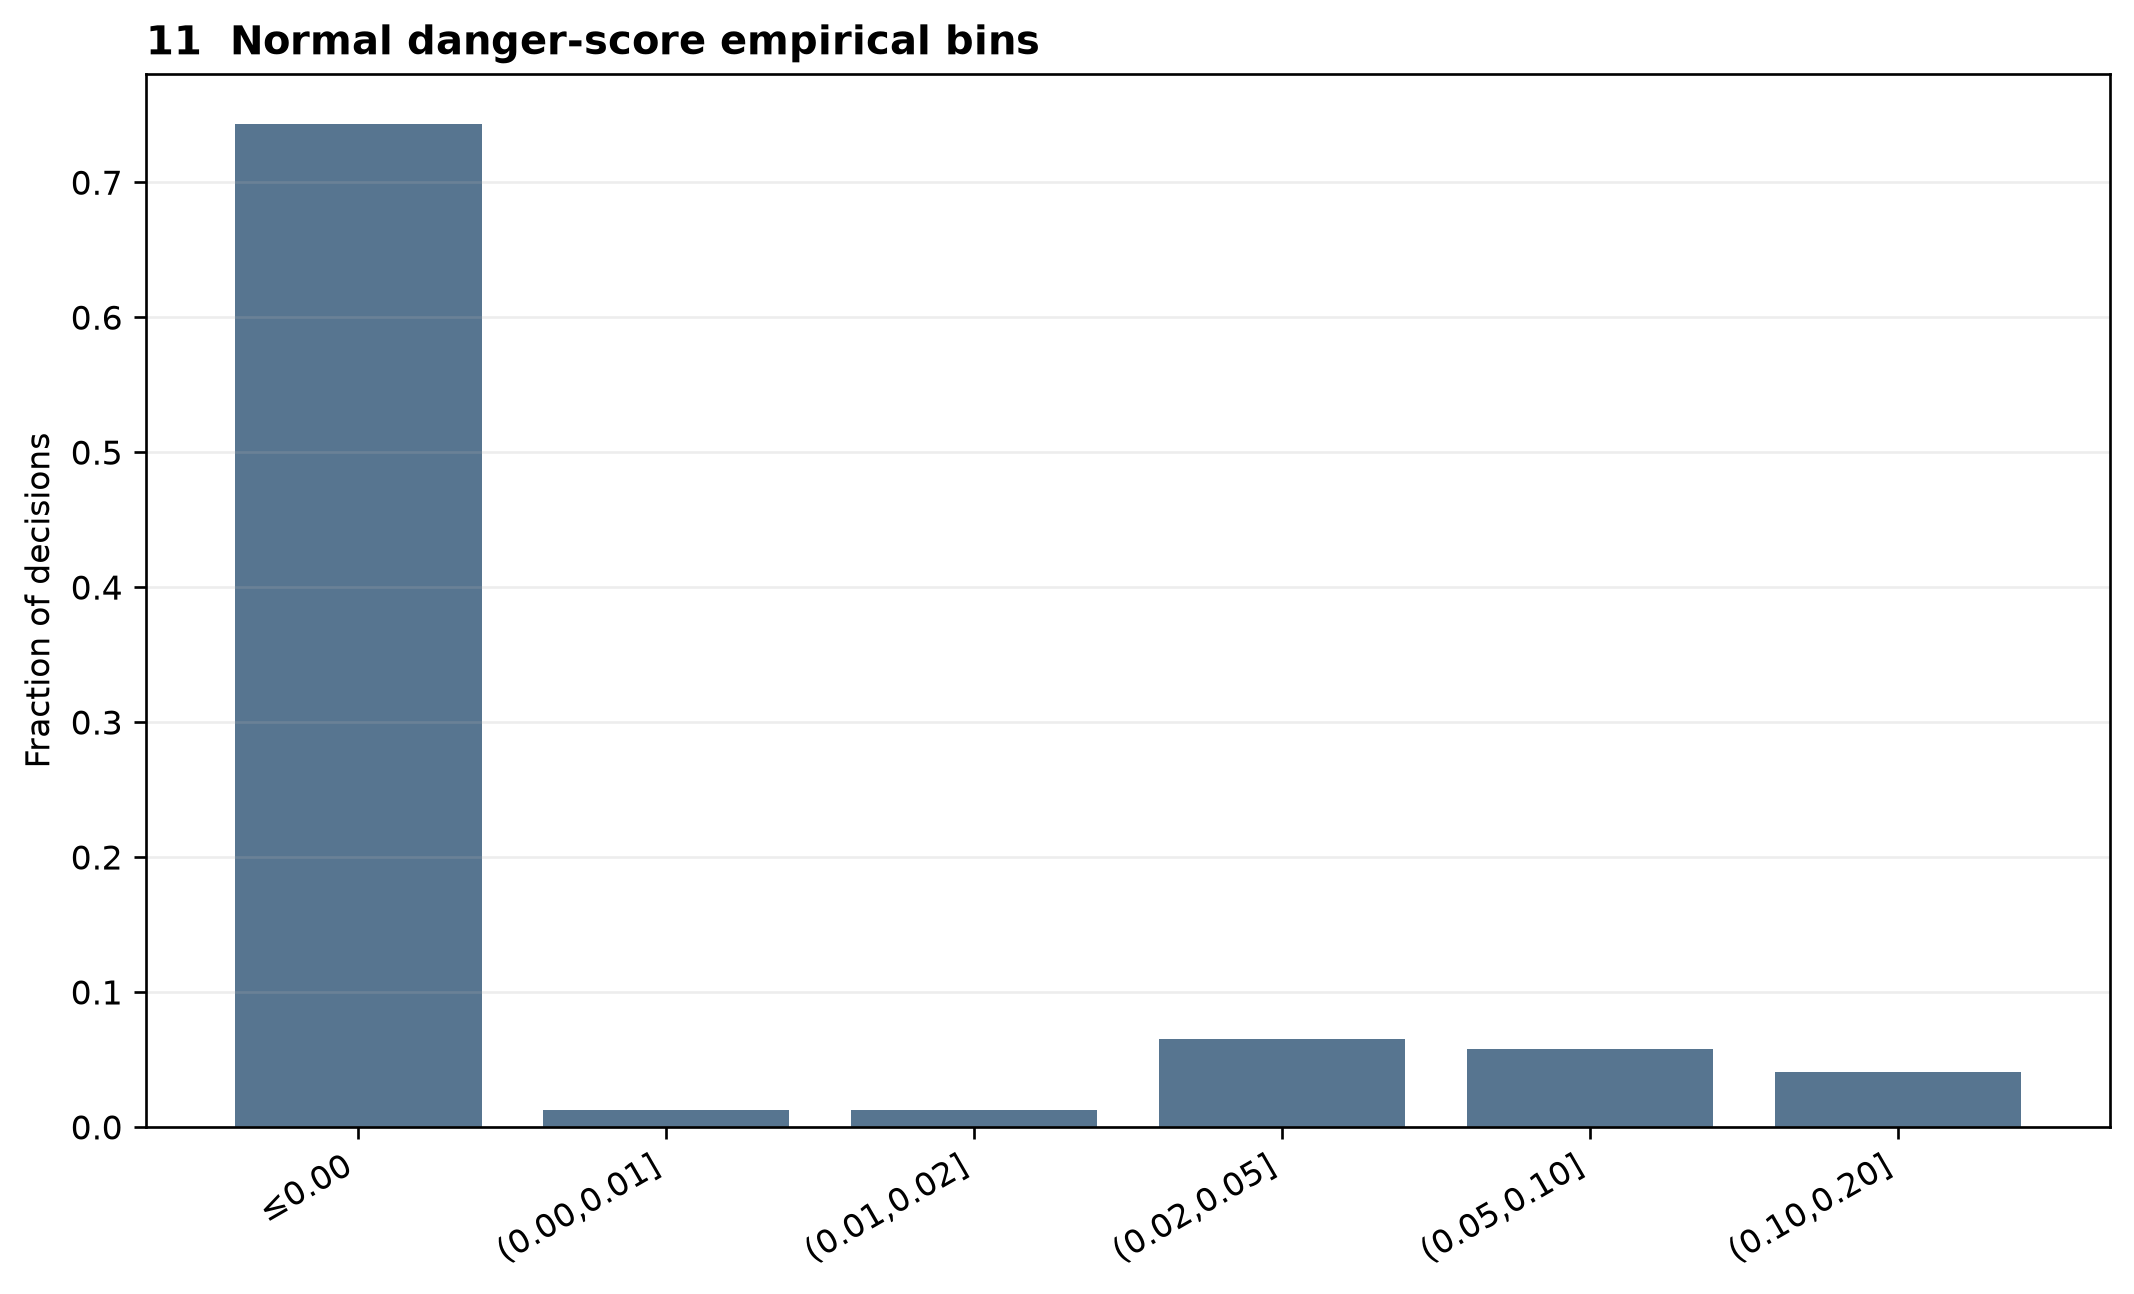
\includegraphics[width=0.90\textwidth]{supplementary_figures/11_gate_score_distribution.png}
\caption{Gate-score interval mass reconstructed from cumulative sweep counts. It is not a raw continuous-score histogram, a distinction needed for reproducible interpretation.}
\label{fig:s11}\end{figure*}

\begin{figure*}[t]\centering
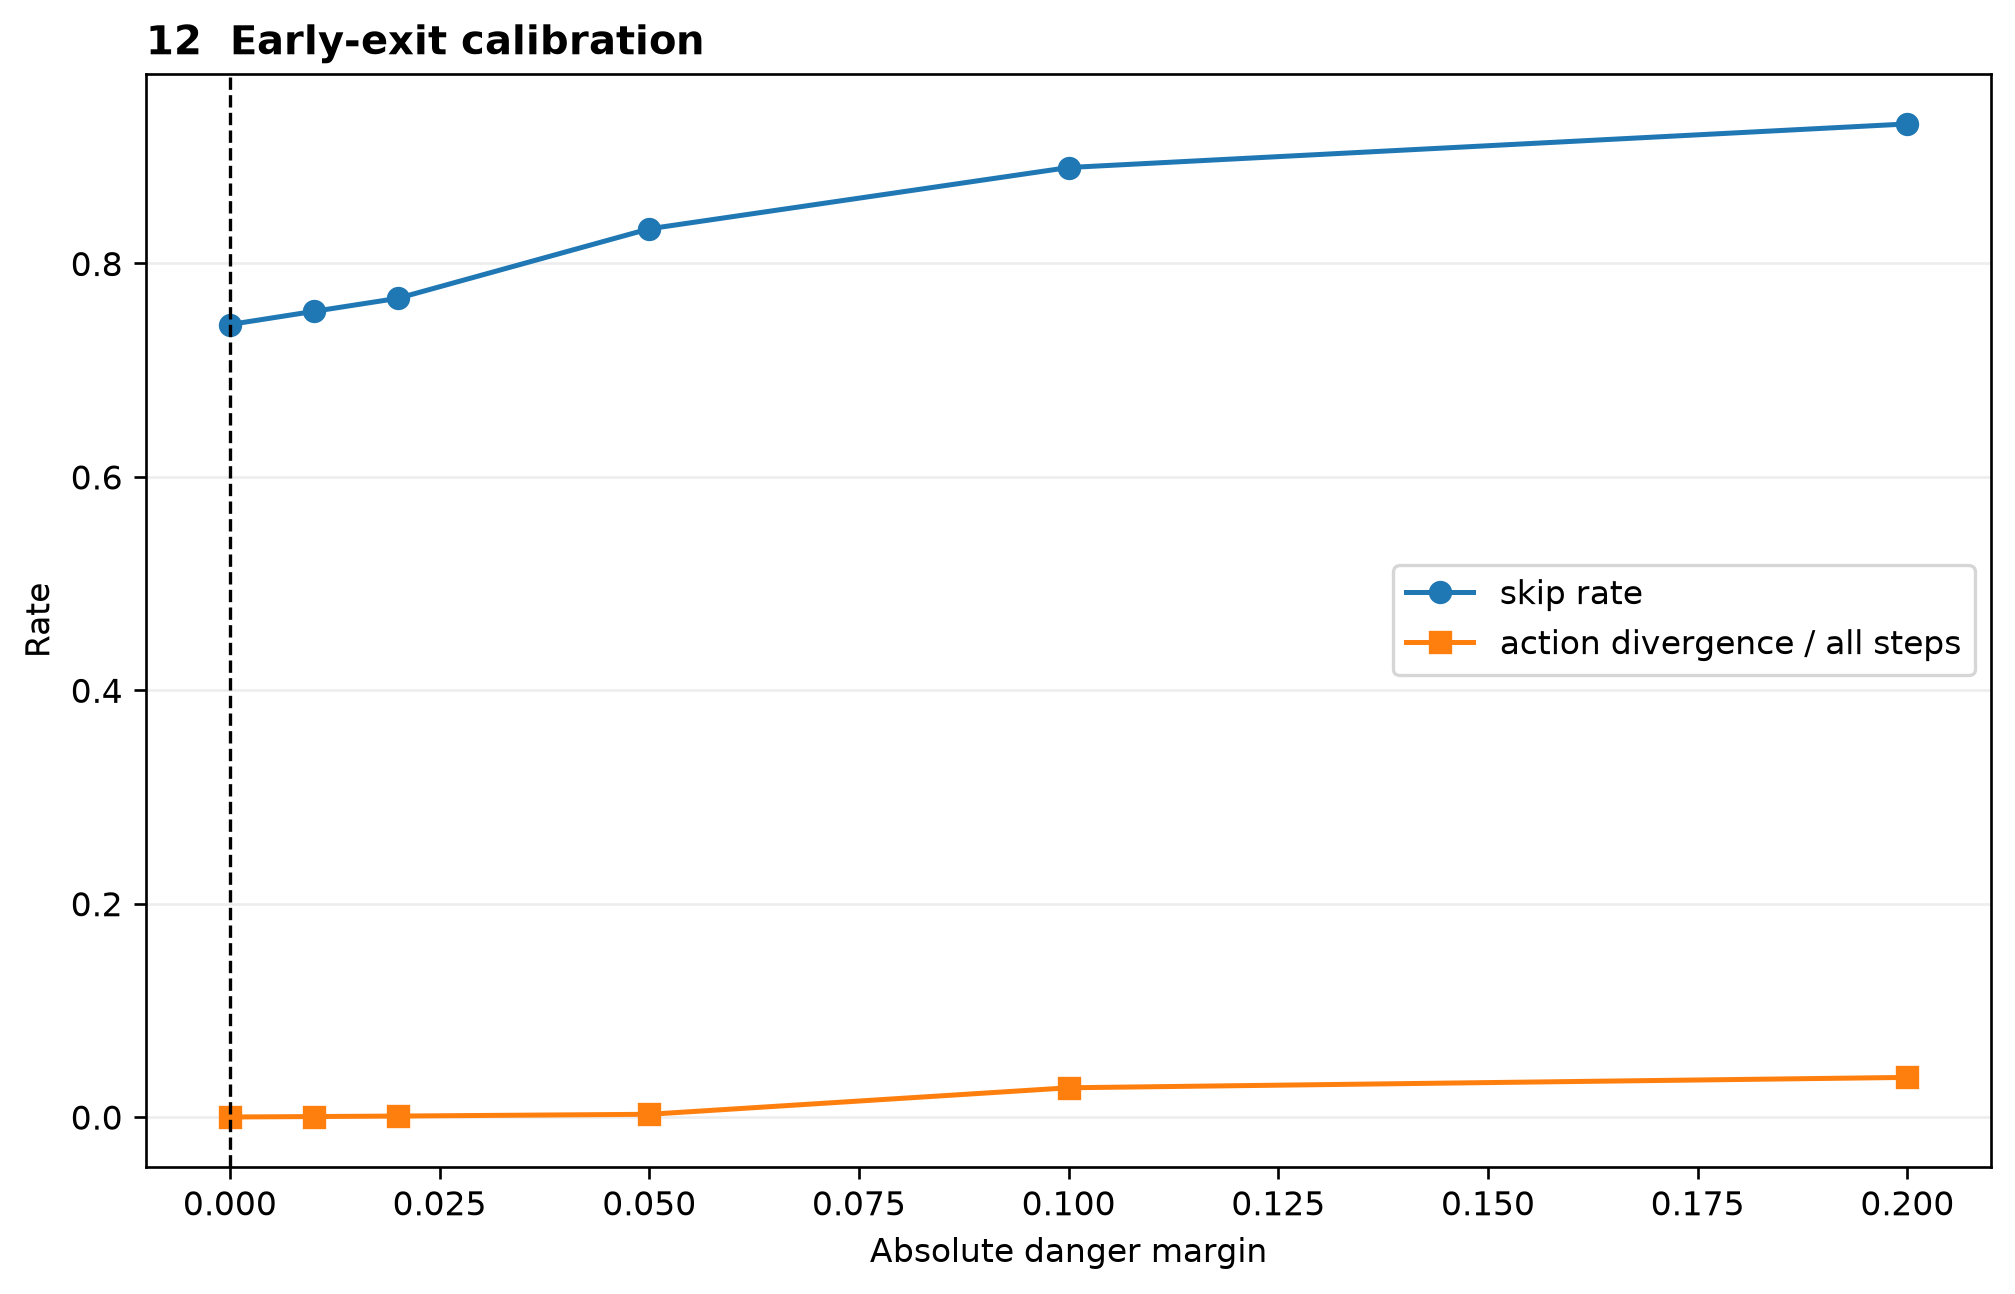
\includegraphics[width=0.90\textwidth]{supplementary_figures/12_gate_calibration.png}
\caption{Early-exit margin sweep. Margin zero is the only tested value with zero observed action divergence over the complete decision trace; positive margins trade additional skipping for mismatches.}
\label{fig:s12}\end{figure*}

\begin{figure*}[t]\centering
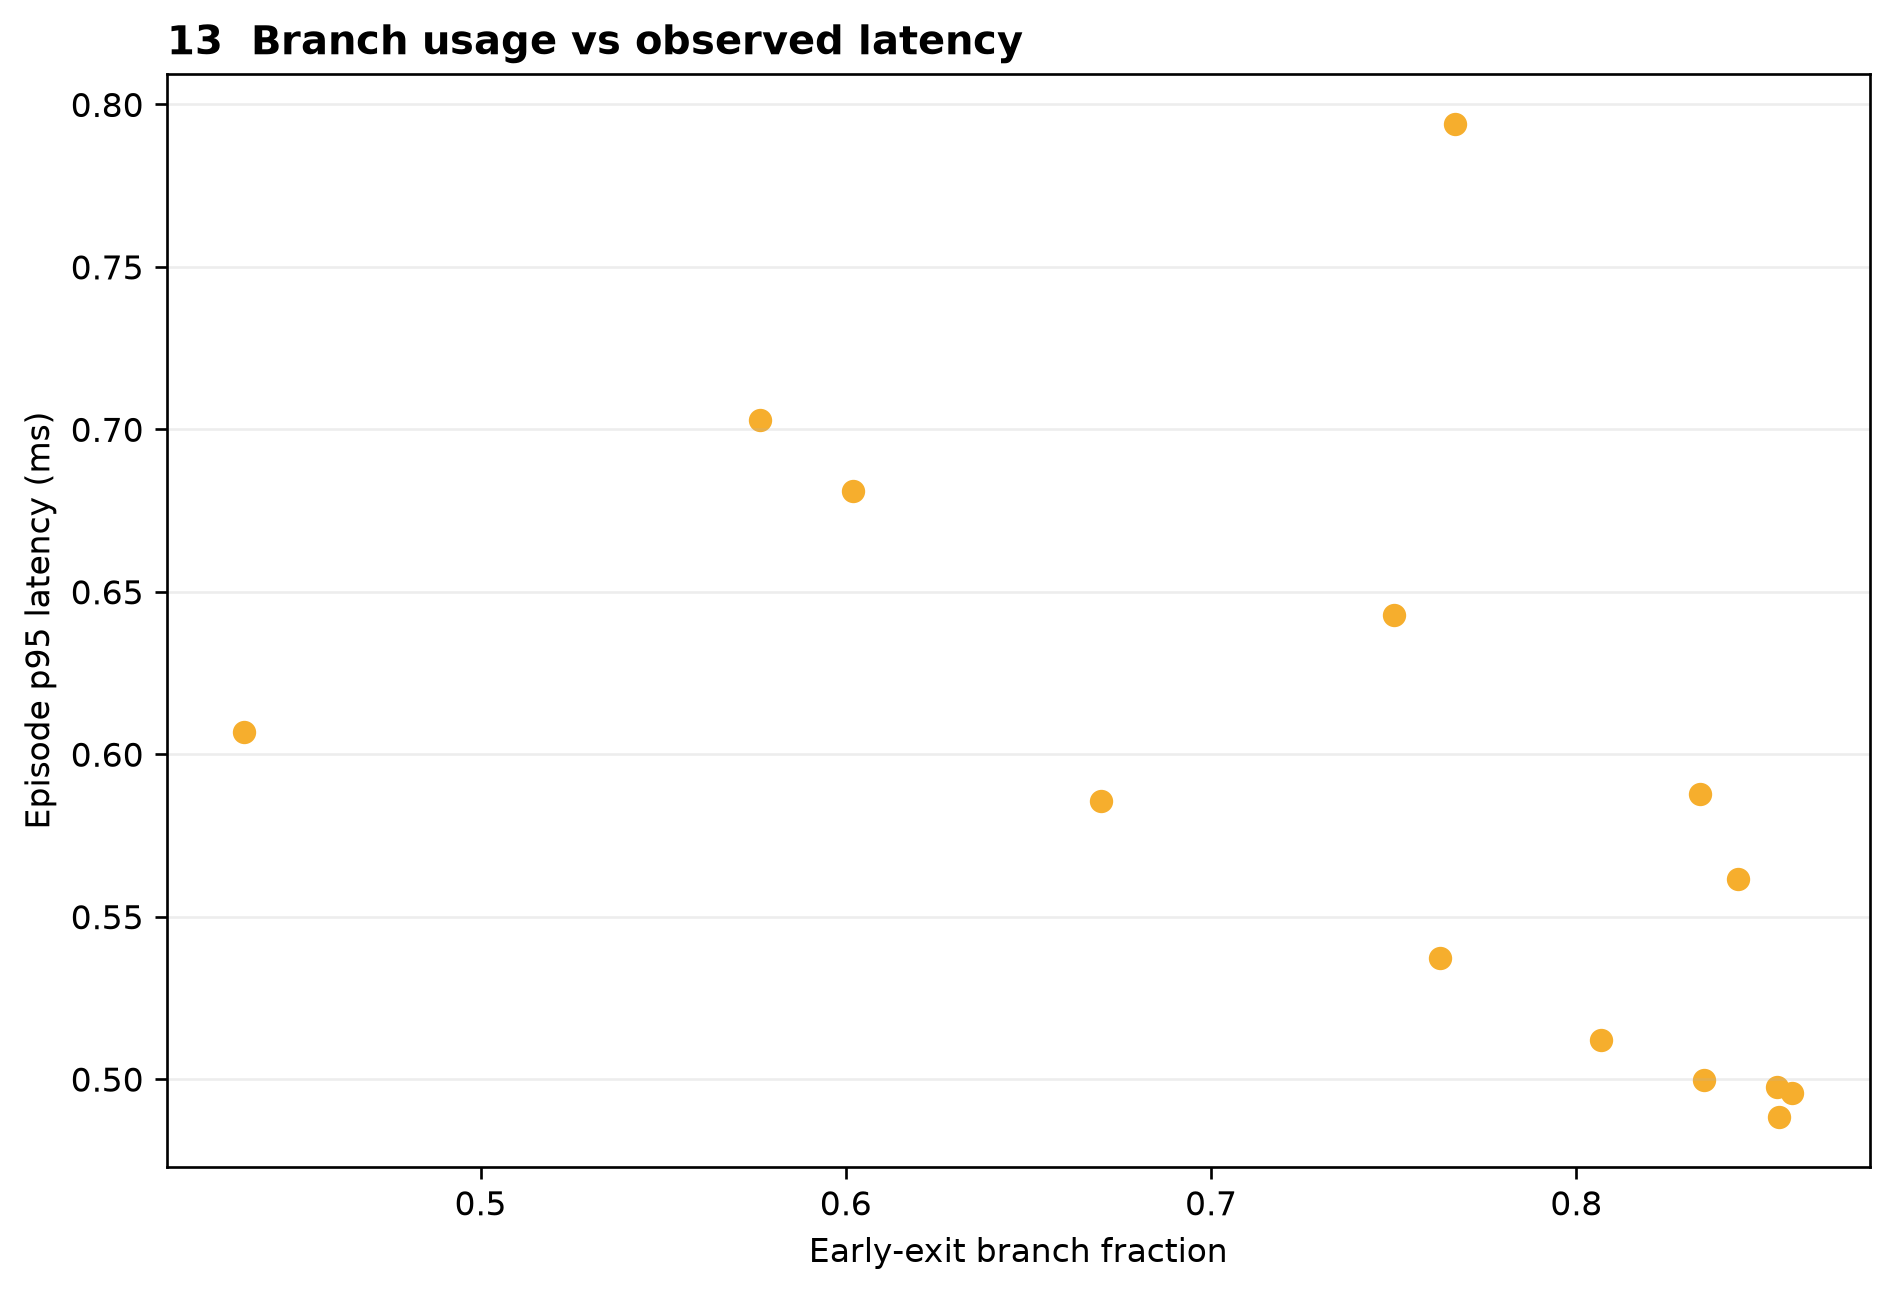
\includegraphics[width=0.90\textwidth]{supplementary_figures/13_branch_usage_latency.png}
\caption{Branch-use rate versus measured latency. A 74.27\% skip rate does not reduce p95 because Python control flow and synchronization exceed the small predictive-branch compute saved.}
\label{fig:s13}\end{figure*}

\begin{figure*}[t]\centering

\includegraphics[width=0.88\textwidth]{supplementary_figures/14_model_footprint.png}
\caption{Parameter and serialized-size comparison. Early Exit shares the DiSwitch weights; Fast-DiSwitch contains 7,011 parameters and is a separately distilled approximate model.}
\label{fig:s14}\end{figure*}

\begin{figure*}[t]\centering

\includegraphics[width=0.88\textwidth]{supplementary_figures/15_policy_input_bytes.png}
\caption{Policy-input memory footprint. This is not radio control overhead; feature acquisition traffic should be instrumented independently on a network implementation.}
\label{fig:s15}\end{figure*}

\begin{figure*}[t]\centering
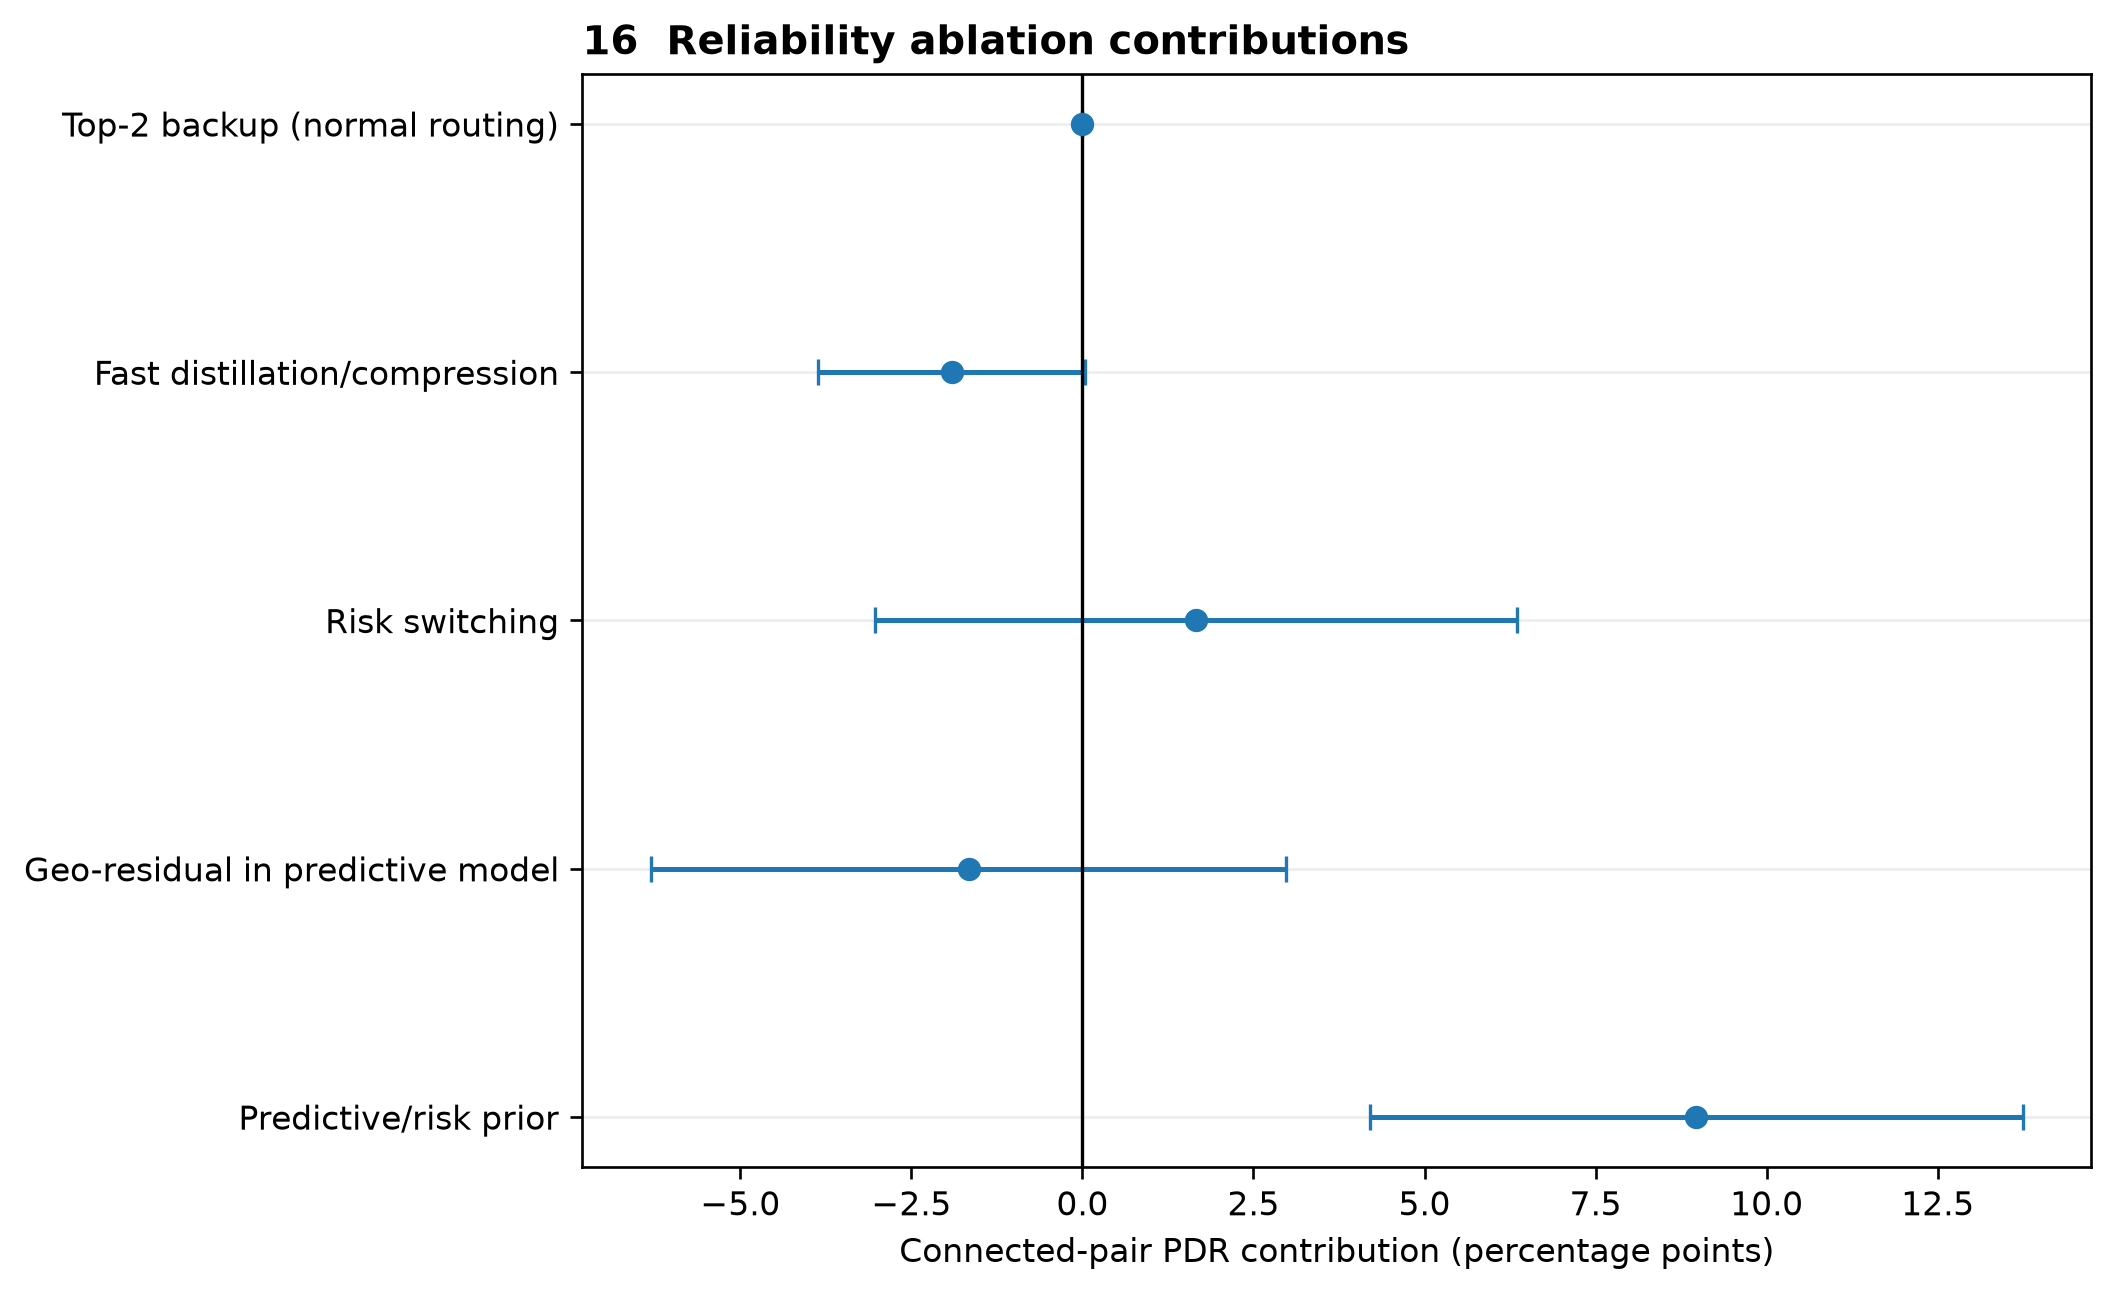
\includegraphics[width=0.92\textwidth]{supplementary_figures/16_ablation_contribution.png}
\caption{Directional ablation contributions with five-seed intervals. The plot separates the normal distilled policy, predictive information, and switching behavior.}
\label{fig:s16}\end{figure*}

\begin{figure*}[t]\centering

\includegraphics[width=0.92\textwidth]{supplementary_figures/17_device_comparison.png}
\caption{Device comparison. The current 2026-09-05 Colab-CLI run is primary; an older A100 bundle is shown only as an independent reproducibility reference and is not pooled with the current run.}
\label{fig:s17}\end{figure*}

\begin{figure*}[t]\centering

\includegraphics[width=\textwidth]{supplementary_figures/18_worst_case_scenario.png}
\caption{Worst-scenario localization. The figure prevents an acceptable macro average from hiding unacceptable OOD or link-loss behavior.}
\label{fig:s18}\end{figure*}

\begin{figure*}[t]\centering

\includegraphics[width=0.90\textwidth]{supplementary_figures/19_early_exit_paired_difference.png}
\caption{Early-Exit paired latency differences across five seeds. The average direction is worse and improvement is not consistent.}
\label{fig:s19}\end{figure*}

\begin{figure*}[t]\centering

\includegraphics[width=0.92\textwidth]{supplementary_figures/20_failed_candidate_tradeoff.png}
\caption{Candidate decision matrix. DiSwitch improves the duplicated legacy execution without an outcome change; buffering is too small; Early Exit is slower; Fast-DiSwitch violates the quality gate.}
\label{fig:s20}\end{figure*}

\section{Latency Tables}

\begin{table*}[t]
\caption{Primary A100 session summary (five checkpoint means).}\label{tab:a100}\small
\begin{tabularx}{\textwidth}{llYYYYY}
\toprule Variant & Device & Mean & p50 & p95 & p99 & Decision \\
\midrule
DiSwitch & CPU & 2.168 & 2.161 & 2.208 & 2.344 & retain \\
Early Exit & CPU & 2.366 & 2.356 & 2.427 & 2.581 & reject \\
Fast-DiSwitch & CPU & 0.812 & 0.814 & 0.847 & 0.927 & quality fail \\
Fast-DiSwitch + Top-2 & CPU & 0.853 & 0.852 & 0.881 & 0.933 & quality unresolved \\
Buffered DiSwitch & CPU & 2.187 & 2.179 & 2.244 & 2.370 & hold \\
Legacy repeated & CPU & 3.698 & 3.687 & 3.775 & 3.935 & superseded \\
DiSwitch & CUDA & 5.671 & 5.648 & 5.836 & 6.101 & retain \\
Early Exit & CUDA & 6.198 & 6.172 & 6.386 & 6.663 & reject \\
Fast-DiSwitch & CUDA & 1.957 & 1.950 & 2.005 & 2.120 & quality fail \\
Fast-DiSwitch + Top-2 & CUDA & 2.040 & 2.032 & 2.092 & 2.183 & quality unresolved \\
Buffered DiSwitch & CUDA & 5.626 & 5.602 & 5.788 & 6.020 & hold \\
Legacy repeated & CUDA & 9.741 & 9.706 & 10.004 & 10.376 & superseded \\
\bottomrule
\end{tabularx}
\end{table*}

\begin{table*}[t]
\caption{Paired CUDA p95 effects relative to DiSwitch. Positive reduction means faster.}\label{tab:paired}\small
\begin{tabularx}{\textwidth}{lYYYY}
\toprule Candidate & p95 reduction & 95\% $t$ CI & Bootstrap 95\% CI & Interpretation \\
\midrule
Early Exit & $-9.42\%$ & [$-10.62$,$-8.22$] & [$-10.22$,$-8.61$] & slower \\
Buffered DiSwitch & $+0.83\%$ & [$+0.21$,$+1.44$] & [$+0.48$,$+1.25$] & too small; CPU reverses \\
Fast-DiSwitch & $+65.65\%$ & [$+65.06$,$+66.24$] & [$+65.24$,$+65.95$] & latency pass, quality fail \\
Fast-DiSwitch + Top-2 & $+64.16\%$ & [$+63.65$,$+64.66$] & [$+63.84$,$+64.50$] & latency pass, quality unresolved \\
\bottomrule
\end{tabularx}
\end{table*}

\section{DiSwitch--Fast-DiSwitch Reliability Gate}

\begin{table*}[t]
\caption{Fast-DiSwitch minus DiSwitch directional paired effects. Higher-is-better metrics use Fast-DiSwitch$-$DiSwitch; lower-is-better metrics reverse the subtraction, so negative always means degradation.}\label{tab:fast}\small
\begin{tabularx}{\textwidth}{lYYYYY}
\toprule Metric & DiSwitch & Fast-DiSwitch & Directional change & 95\% CI & Gate \\
\midrule
Connected-pair PDR & 0.90529 & 0.88720 & $-0.01809$ & \shortstack{$-0.03606$ to\\$-0.00011$} & fail \\
Deadline ratio & 0.83764 & 0.81500 & $-0.02264$ & \shortstack{$-0.04625$ to\\$+0.00096$} & fail \\
p95 success delay & 4.2643 & 4.4864 & $-0.2221$ & \shortstack{$-0.4208$ to\\$-0.0235$} & fail \\
Energy/delivered proxy & 2.2279 & 2.3694 & $-0.1415$ & \shortstack{$-0.2799$ to\\$-0.0031$} & fail \\
\bottomrule
\end{tabularx}
\end{table*}

The connected-PDR interval lies entirely below zero and its lower bound is far below the allowed $-0.005$. Fast-DiSwitch therefore cannot be called statistically equivalent or non-inferior to DiSwitch. The deadline interval overlaps zero at its upper edge, but its lower edge independently violates the gate. The delay and energy directions reinforce the rejection.

\section{Operator-Profile Interpretation}

The DiSwitch profile contains 1,050 \texttt{\seqsplit{aten::\_local\_scalar\_dense}} events and the same number of device-to-host copies over 30 calls. Early Exit contains 1,140 of each; Fast-DiSwitch contains 300; Fast-DiSwitch+Top-2 contains 330. The counts are evidence of synchronization frequency, not time percentages for the primary benchmark. DiSwitch also shows Boolean reductions such as \texttt{aten::all} and \texttt{aten::any}, which are consistent with action-mask and gate logic.

This evidence motivates three implementation hypotheses: (i) preserve gate and action extraction as tensors until the final API boundary; (ii) replace Python branching with a runtime-native conditional graph; and (iii) combine small elementwise and reduction operations where the deployment compiler can do so without altering masks or threshold comparisons. Any optimized graph must pass logit/action replay or the same routing-quality gate used for Fast-DiSwitch.

\section{Reproduction Checklist}

\begin{enumerate}
\item Check out the recorded source commit and verify that no untracked implementation changes remain.
\item Verify SHA-256 for the source bundle and five DiSwitch/Fast-DiSwitch checkpoint archives.
\item Run the full routing evaluation with seeds 42, 77, 123, 314, and 2718; 14 scenario definitions; and 200 episodes per cell.
\item Verify 14,000 episodes per method, 112,000 combined rows, finite metrics, valid actions, and mask compliance.
\item Aggregate per seed and scenario before forming 14-scenario macro values; preserve N/A successful-delay cells.
\item Run CPU and CUDA latency variants in one session, one CPU thread, batch one, 50 warm-ups, and 2,000 repetitions per checkpoint.
\item Synchronize CUDA before and after the end-to-end timing region; keep cold start separate.
\item Compute matched-seed effects, Student-$t$ intervals, deterministic bootstrap intervals, exact sign-flip tests, and Holm-adjusted comparisons.
\item Run operator profiling separately and do not merge profiler timings with primary latency values.
\item Regenerate all figures from the copied CSV sources and compare the figure manifest.
\end{enumerate}

\section{Reporting Checklist for Submission}

Before submission, the authors should verify the current IEEE Access template version, decide on a public repository/DOI or a defensible restricted-access statement, add the precise simulator license, state the compute resource provider, and determine whether adapted baseline code can be released. A target-device experiment is strongly recommended. If it cannot be completed, the title, abstract, and conclusion should retain the term ``deployment-oriented'' rather than ``deployed'' or ``real-time onboard.''

\EOD
\end{document}
